\appendix
\section{Generalized Object Detection Benchmarks}
We present the full benchmark results of PASCAL VOC (Table~\ref{tab:voc_bench}) and COCO
(Table~\ref{tab:coco_bench}) on the revised benchmark used in this work. We report the average AP, AP50 and AP75 for all the classes, base classes only, and novel classes only in the tables. For each evaluation metric, we report the average value of $n$ repeated runs with different groups of randomly sampled training shots (30 for PASCAL VOC and 10 for COCO) as well as the 95\% confidence interval estimate of the mean values.  The 95\% confidence interval is calculated by 
\begin{equation}
    95\% \; CI = 1.96 \cdot \frac{s}{\sqrt{n}},
\end{equation}
where 1.96 is the $Z$-value, $s$ is the standard deviation, and $n$ is the number of repeated runs.

We compare two of our methods, one using a FC-based classifier (\texttt{\model w/fc}) and one using a cosine similarity based classifier (\texttt{\model w/cos}). We also compare against a fine-tuning baseline \texttt{FRCN+ft-full} and against FSRW~\cite{kang2019few} using their released code on PASCAL VOC shown in Table~\ref{tab:voc_bench}. 

As shown in Table~\ref{tab:voc_bench},
\texttt{\model w/cos} is able to significantly outperform \texttt{\model w/fc} in overall AP across most splits and shots.
We observe that using a cosine similarity based classifier can achieve much higher accuracy on base classes, especially in higher shots.
On split 1 and 3, \texttt{\model w/cos} is able to outperform \texttt{\model w/fc} by over 3 points on bAP on 5 and 10 shots.
Across all shots in split 1, \texttt{\model w/cos} consistently outperforms \texttt{\model w/fc} on nAP75 by over 2 points in the novel classes. 

Moreover, the AP of our models is usually over 10 points higher than that of \texttt{FRCN+ft-full} and FSRW on all settings. Note that FSRW uses YOLOv2 as the base object detector, while we are using Faster R-CNN. ~\citet{wang2019meta} shows that there are only about 2 points of difference when using a one or two-stage detector. Therefore, our improvements should still be significant despite the difference in the base detector.

We evaluate on COCO over six different number of shots $K=1,2,3,5,10,30$ shown in Table~\ref{tab:coco_bench}.
Although the differences are less significant than on PASCAL VOC, similar observations can be made about accuracy on base classes and novel classes.

\begin{table*}[!h]
\centering
\footnotesize
\setlength{\tabcolsep}{0.4em}
\caption{Generalized object detection benchmarks on PASCAL VOC. For each metric, we report the average and 95\% confidence interval computed over 30 random samples. \vspace{1mm}}
\adjustbox{width=\linewidth}{
\begin{tabular}{c|c|c|ccc|ccc|ccc}
\toprule
\multirow{2}{*}{Split} & \multirow{2}{*}{\# shots} &\multirow{2}{*}{Method} &  \multicolumn{3}{c|}{Overall}  &\multicolumn{3}{c|}{Base class} & \multicolumn{3}{c}{Novel class} \\ \cmidrule{4-12}
& & & AP & AP50 & AP75 & bAP & bAP50 & bAP75 & nAP & nAP50 & nAP75 \\ \midrule
\multirow{21}{*}{Split 1} & 
\multirow{4}{*}{1}
    & FSRW~\cite{kang2019few} & 27.6 $ \pm $ 0.5 & 50.8 $ \pm $ 0.9 & 26.5 $ \pm $ 0.6 & 34.1 $ \pm $ 0.5 & 62.9 $ \pm $ 0.9 & 32.6 $ \pm $ 0.5 & 8.0 $ \pm $ 1.0 & 14.2 $ \pm $ 1.7 & 7.9 $ \pm $ 1.1\\
    & & FRCN+ft-full & 30.2$\pm$0.6 & 49.4$\pm$0.7 & 32.2$\pm$0.9 & 38.2$\pm$0.8 & 62.6$\pm$1.0 & 40.8$\pm$1.1 & 6.0$\pm$0.7 & 9.9$\pm$1.2 & 6.3$\pm$0.8\\
     & & {\model w/fc} & 39.6$\pm$0.5 & 63.5$\pm$0.7 & 43.2$\pm$0.7 & 48.7$\pm$0.7 & 77.1$\pm$0.7 & 53.7$\pm$1.0 & 12.2$\pm$1.6 & 22.9$\pm$2.5 & 11.6$\pm$1.9 \\
    & &\cellcolor{Gray} {\model w/cos} & \cellcolor{Gray}40.6$\pm$0.5 & \cellcolor{Gray}64.5$\pm$0.6 & \cellcolor{Gray}44.7$\pm$0.6 & \cellcolor{Gray}49.4$\pm$0.4 & \cellcolor{Gray}77.6$\pm$0.2 & \cellcolor{Gray}54.8$\pm$0.5 & \cellcolor{Gray}14.2$\pm$1.4 &\cellcolor{Gray} 25.3$\pm$2.2 & \cellcolor{Gray}14.2$\pm$1.8 \\ \cmidrule{2-12}
    & \multirow{4}{*}{2} & FSRW~\cite{kang2019few} & 
    28.7$\pm$0.4&52.2$\pm$0.6&27.7$\pm$0.5&33.9$\pm$0.4&61.8$\pm$0.5&32.7$\pm$0.5&13.2$\pm$1.0&23.6$\pm$1.7&12.7$\pm$1.1 \\
    & & FRCN+ft-full & 30.5$\pm$0.6 & 49.4$\pm$0.8 & 32.6$\pm$0.7 & 37.3$\pm$0.7 & 60.7$\pm$1.0 & 40.1$\pm$0.9 & 9.9$\pm$0.9 & 15.6$\pm$1.4 & 10.3$\pm$1.0 \\
    & & {\model w/fc} & 40.5$\pm$0.5 & 65.5$\pm$0.7 & 43.8$\pm$0.7 & 47.8$\pm$0.7 & 75.8$\pm$0.7 & 52.2$\pm$1.0 & 18.9$\pm$1.5 & 34.5$\pm$2.4 & 18.4$\pm$1.9  \\
    & &\cellcolor{Gray} {\model w/cos} & \cellcolor{Gray}42.6$\pm$0.3 & \cellcolor{Gray} 67.1$\pm$0.4 & \cellcolor{Gray}47.0$\pm$0.4 &\cellcolor{Gray} 49.6$\pm$0.3 & \cellcolor{Gray}77.3$\pm$0.2 & \cellcolor{Gray}55.0$\pm$0.4 & \cellcolor{Gray}21.7$\pm$1.0 & \cellcolor{Gray}36.4$\pm$1.6 & \cellcolor{Gray}22.8$\pm$1.3  \\ \cmidrule{2-12}
    & \multirow{4}{*}{3} & FSRW~\cite{kang2019few} & 29.5$\pm$0.3&53.3$\pm$0.6&28.6$\pm$0.4&33.8$\pm$0.3&61.2$\pm$0.6&32.7$\pm$0.4&16.8$\pm$0.9&29.8$\pm$1.6&16.5$\pm$1.0 \\
    & & FRCN+ft-full & 31.8$\pm$0.5 & 51.4$\pm$0.8 & 34.2$\pm$0.6 & 37.9$\pm$0.5 & 61.3$\pm$0.7 & 40.7$\pm$0.6 & 13.7$\pm$1.0 & 21.6$\pm$1.6 & 14.8$\pm$1.1 \\
    & & {\model w/fc} & 41.8$\pm$0.9 & 67.1$\pm$0.9 & 45.4$\pm$1.2 & 48.2$\pm$0.9 & 76.0$\pm$0.9 & 53.1$\pm$1.2 & 22.6$\pm$1.2 & 40.4$\pm$1.7 & 22.4$\pm$1.7  \\
    & & \cellcolor{Gray}{\model w/cos} &\cellcolor{Gray} 43.7$\pm$0.3 &\cellcolor{Gray} 68.5$\pm$0.4 & \cellcolor{Gray}48.3$\pm$0.4 & \cellcolor{Gray}49.8$\pm$0.3 & \cellcolor{Gray}77.3$\pm$0.2 & \cellcolor{Gray}55.4$\pm$0.4 & \cellcolor{Gray}25.4$\pm$0.9 & \cellcolor{Gray}42.1$\pm$1.5 & \cellcolor{Gray}27.0$\pm$1.2  \\ \cmidrule{2-12}
    & \multirow{4}{*}{5} & FSRW~\cite{kang2019few} & 30.4$\pm$0.3&54.6$\pm$0.5&29.6$\pm$0.4&33.7$\pm$0.3&60.7$\pm$0.4&32.8$\pm$0.4&20.6$\pm$0.8&36.5$\pm$1.4&20.0$\pm$0.9 \\
    & & FRCN+ft-full & 32.7$\pm$0.5 & 52.5$\pm$0.8 & 35.0$\pm$0.6 & 37.6$\pm$0.4 & 60.6$\pm$0.6 & 40.3$\pm$0.5 & 17.9$\pm$1.1 & 28.0$\pm$1.7 & 19.2$\pm$1.3 \\
    & & {\model w/fc} & 41.9$\pm$0.6 & 68.0$\pm$0.7 & 45.0$\pm$0.8 & 47.2$\pm$0.6 & 75.1$\pm$0.6 & 51.5$\pm$0.8 & 25.9$\pm$1.0 & 46.7$\pm$1.4 & 25.3$\pm$1.2  \\
    & &\cellcolor{Gray} {\model w/cos} &\cellcolor{Gray} 44.8$\pm$0.3 & \cellcolor{Gray}70.1$\pm$0.4 &\cellcolor{Gray} 49.4$\pm$0.4 &\cellcolor{Gray} 50.1$\pm$0.2 &\cellcolor{Gray} 77.4$\pm$0.3 &\cellcolor{Gray} 55.6$\pm$0.3 &\cellcolor{Gray} 28.9$\pm$0.8 & \cellcolor{Gray}47.9$\pm$1.2 & \cellcolor{Gray}30.6$\pm$1.0  \\ \cmidrule{2-12}
    & \multirow{3}{*}{10} & FRCN+ft-full & 33.3$\pm$0.4 & 53.8$\pm$0.6 & 35.5$\pm$0.4 & 36.8$\pm$0.4 & 59.8$\pm$0.6 & 39.2$\pm$0.4 & 22.7$\pm$0.9 & 35.6$\pm$1.5 & 24.4$\pm$1.0 \\
    & & {\model w/fc} & 42.8$\pm$0.3 & 69.5$\pm$0.4 & 46.0$\pm$0.4 & 47.3$\pm$0.3 & 75.4$\pm$0.3 & 51.6$\pm$0.4 & 29.3$\pm$0.7 & 52.0$\pm$1.1 & 29.0$\pm$0.9  \\
    & &\cellcolor{Gray} {\model w/cos} & \cellcolor{Gray}45.8$\pm$0.2 & \cellcolor{Gray}71.3$\pm$0.3 & \cellcolor{Gray}50.4$\pm$0.3 &\cellcolor{Gray} 50.4$\pm$0.2 & \cellcolor{Gray}77.5$\pm$0.2 &\cellcolor{Gray} 55.9$\pm$0.3 & \cellcolor{Gray}32.0$\pm$0.6 & \cellcolor{Gray}52.8$\pm$1.0 & \cellcolor{Gray}33.7$\pm$0.7  \\ \midrule
\multirow{21}{*}{Split 2} & \multirow{4}{*}{1} & FSRW~\cite{kang2019few} &
    28.4$\pm$0.5&51.7$\pm$0.9&27.3$\pm$0.6&35.7$\pm$0.5&64.8$\pm$0.9&34.6$\pm$0.7&6.3$\pm$0.9&12.3$\pm$1.9&5.5$\pm$0.7 \\
    & & FRCN+ft-full & 30.3$\pm$0.5 & 49.7$\pm$0.5 & 32.3$\pm$0.7 & 38.8$\pm$0.6 & 63.2$\pm$0.7 & 41.6$\pm$0.9 & 5.0$\pm$0.6 & 9.4$\pm$1.2 & 4.5$\pm$0.7 \\
    & & {\model w/fc} & 36.2$\pm$0.8 & 59.6$\pm$0.9 & 38.7$\pm$1.0 & 45.6$\pm$0.9 & 73.8$\pm$0.9 & 49.4$\pm$1.2 & 8.1$\pm$1.2 & 16.9$\pm$2.3 & 6.6$\pm$1.1  \\
    & &\cellcolor{Gray} {\model w/cos} & \cellcolor{Gray}36.7$\pm$0.6 &\cellcolor{Gray} 59.9$\pm$0.8 &\cellcolor{Gray} 39.3$\pm$0.8 &\cellcolor{Gray} 45.9$\pm$0.7 & \cellcolor{Gray}73.8$\pm$0.8 &\cellcolor{Gray} 49.8$\pm$1.1 & \cellcolor{Gray}9.0$\pm$1.2 & \cellcolor{Gray}18.3$\pm$2.4 &\cellcolor{Gray} 7.8$\pm$1.2 \\ \cmidrule{2-12}
    & \multirow{4}{*}{2} & FSRW~\cite{kang2019few} & 
    29.4$\pm$0.3&53.1$\pm$0.6&28.5$\pm$0.4&35.8$\pm$0.4&64.2$\pm$0.6&35.1$\pm$0.5&9.9$\pm$0.7&19.6$\pm$1.3&8.8$\pm$0.6 \\
    & & FRCN+ft-full & 30.7$\pm$0.5 & 49.7$\pm$0.7 & 32.9$\pm$0.6 & 38.4$\pm$0.5 & 61.6$\pm$0.7 & 41.4$\pm$0.7 & 7.7$\pm$0.8 & 13.8$\pm$1.4 & 7.4$\pm$0.8 \\
    & &{\model w/fc} & 38.5$\pm$0.5 & 62.8$\pm$0.6 & 41.2$\pm$0.6 & 46.9$\pm$0.5 & 74.9$\pm$0.5 & 51.2$\pm$0.7 & 13.1$\pm$1.0 & 26.4$\pm$1.9 & 11.3$\pm$1.1  \\
    & & \cellcolor{Gray}{\model w/cos} & \cellcolor{Gray}39.0$\pm$0.4 & \cellcolor{Gray}63.0$\pm$0.5 & \cellcolor{Gray}42.1$\pm$0.6 & \cellcolor{Gray}47.3$\pm$0.4 & \cellcolor{Gray}74.9$\pm$0.4 &\cellcolor{Gray} 51.9$\pm$0.7 &\cellcolor{Gray} 14.1$\pm$0.9 &\cellcolor{Gray} 27.5$\pm$1.6 &\cellcolor{Gray} 12.7$\pm$1.0  \\ \cmidrule{2-12}
    & \multirow{4}{*}{3} & FSRW~\cite{kang2019few} & 29.9$\pm$0.3&53.9$\pm$0.4&29.0$\pm$0.4&35.7$\pm$0.3&63.5$\pm$0.4&35.1$\pm$0.4&12.5$\pm$0.7&25.1$\pm$1.4&10.4$\pm$0.7 \\
    & & FRCN+ft-full & 31.1$\pm$0.3 & 50.1$\pm$0.5 & 33.2$\pm$0.5 & 38.1$\pm$0.4 & 61.0$\pm$0.6 & 41.2$\pm$0.5 & 9.8$\pm$0.9 & 17.4$\pm$1.6 & 9.4$\pm$1.0 \\
    & &{\model w/fc} & 39.4$\pm$0.4 & 64.2$\pm$0.5 & 42.0$\pm$0.5 & 47.5$\pm$0.4 & 75.4$\pm$0.5 & 51.7$\pm$0.6 & 15.2$\pm$0.8 & 30.5$\pm$1.5 & 13.1$\pm$0.8  \\
    & & \cellcolor{Gray}{\model w/cos} & \cellcolor{Gray}40.1$\pm$0.3 &\cellcolor{Gray} 64.5$\pm$0.5 &\cellcolor{Gray} 43.3$\pm$0.4 &\cellcolor{Gray} 48.1$\pm$0.3 & \cellcolor{Gray}75.6$\pm$0.4 & \cellcolor{Gray}52.9$\pm$0.5 & \cellcolor{Gray}16.0$\pm$0.8 & \cellcolor{Gray}30.9$\pm$1.6 & \cellcolor{Gray}14.4$\pm$0.9  \\ \cmidrule{2-12}
    & \multirow{4}{*}{5} & FSRW~\cite{kang2019few} & 30.4$\pm$0.4&54.6$\pm$0.5&29.5$\pm$0.5&35.3$\pm$0.3&62.4$\pm$0.4&34.9$\pm$0.5&15.7$\pm$0.8&31.4$\pm$1.5&13.3$\pm$0.9 \\
    & & FRCN+ft-full & 31.5$\pm$0.3 & 50.8$\pm$0.7 & 33.6$\pm$0.4 & 37.9$\pm$0.4 & 60.4$\pm$0.6 & 40.8$\pm$0.5 & 12.4$\pm$0.9 & 21.9$\pm$1.5 & 12.1$\pm$0.9 \\
    & &{\model w/fc} & 40.0$\pm$0.4 & 65.1$\pm$0.5 & 42.6$\pm$0.5 & 47.5$\pm$0.4 & 75.3$\pm$0.5 & 51.6$\pm$0.5 & 17.5$\pm$0.7 & 34.6$\pm$1.1 & 15.5$\pm$0.9  \\
    & & \cellcolor{Gray}{\model w/cos} & \cellcolor{Gray}40.9$\pm$0.4 & \cellcolor{Gray}65.7$\pm$0.5 & \cellcolor{Gray}44.1$\pm$0.5 & \cellcolor{Gray}48.6$\pm$0.4 &\cellcolor{Gray} 76.2$\pm$0.4 & \cellcolor{Gray}53.3$\pm$0.5 & \cellcolor{Gray}17.8$\pm$0.8 &\cellcolor{Gray} 34.1$\pm$1.4 & \cellcolor{Gray}16.2$\pm$1.0  \\ \cmidrule{2-12}
    & \multirow{3}{*}{10} & FRCN+ft-full & 32.2$\pm$0.3 & 52.3$\pm$0.4 & 34.1$\pm$0.4 & 37.2$\pm$0.3 & 59.8$\pm$0.4 & 39.9$\pm$0.4 & 17.0$\pm$0.8 & 29.8$\pm$1.4 & 16.7$\pm$0.9 \\
    & & {\model w/fc} & 41.3$\pm$0.2 & 67.0$\pm$0.3 & 44.0$\pm$0.3 & 48.3$\pm$0.2 & 76.1$\pm$0.3 & 52.7$\pm$0.4 & 20.2$\pm$0.5 & 39.7$\pm$0.9 & 18.0$\pm$0.7  \\
    & & \cellcolor{Gray}{\model w/cos} & \cellcolor{Gray}42.3$\pm$0.3 &\cellcolor{Gray} 67.6$\pm$0.4 &\cellcolor{Gray} 45.7$\pm$0.3 &\cellcolor{Gray} 49.4$\pm$0.2 & \cellcolor{Gray}76.9$\pm$0.3 & \cellcolor{Gray}54.5$\pm$0.3 &\cellcolor{Gray} 20.8$\pm$0.6 &\cellcolor{Gray} 39.5$\pm$1.1 & \cellcolor{Gray}19.2$\pm$0.6  \\ \midrule
\multirow{21}{*}{Split 3} & \multirow{4}{*}{1} & FSRW~\cite{kang2019few} &
27.5$\pm$0.6&50.0$\pm$1.0&26.8$\pm$0.7&34.5$\pm$0.7&62.5$\pm$1.2&33.5$\pm$0.7&6.7$\pm$1.0&12.5$\pm$1.6&6.4$\pm$1.0 \\
    & & FRCN+ft-full & 30.8$\pm$0.6 & 49.8$\pm$0.8 & 32.9$\pm$0.8 & 39.6$\pm$0.8 & 63.7$\pm$1.0 & 42.5$\pm$0.9 & 4.5$\pm$0.7 & 8.1$\pm$1.3 & 4.2$\pm$0.7 \\
    & & {\model w/fc} & 39.0$\pm$0.6 & 62.3$\pm$0.7 & 42.1$\pm$0.8 & 49.5$\pm$0.8 & 77.8$\pm$0.8 & 54.0$\pm$1.0 & 7.8$\pm$1.1 & 15.7$\pm$2.1 & 6.5$\pm$1.0 \\
    & & \cellcolor{Gray}{\model w/cos} & \cellcolor{Gray}40.1$\pm$0.3 &\cellcolor{Gray} 63.5$\pm$0.6 &\cellcolor{Gray} 43.6$\pm$0.5 &\cellcolor{Gray} 50.2$\pm$0.4 & \cellcolor{Gray}78.7$\pm$0.2 & \cellcolor{Gray}55.1$\pm$0.5 & \cellcolor{Gray}9.6$\pm$1.1 & \cellcolor{Gray}17.9$\pm$2.0 &\cellcolor{Gray} 9.1$\pm$1.2  \\ \cmidrule{2-12}
    & \multirow{4}{*}{2} & FSRW~\cite{kang2019few} & 28.7$\pm$0.4&51.8$\pm$0.7&28.1$\pm$0.5&34.5$\pm$0.4&62.0$\pm$0.7&34.0$\pm$0.5&11.3$\pm$0.7&21.3$\pm$1.0&10.6$\pm$0.8 \\
    & & FRCN+ft-full & 31.3$\pm$0.5 & 50.2$\pm$0.9 & 33.5$\pm$0.6 & 39.1$\pm$0.5 & 62.4$\pm$0.9 & 42.0$\pm$0.7 & 8.0$\pm$0.8 & 13.9$\pm$1.4 & 7.9$\pm$0.9 \\
    & &{\model w/fc} & 41.1$\pm$0.6 & 65.1$\pm$0.7 & 44.3$\pm$0.7 & 50.1$\pm$0.7 & 77.7$\pm$0.7 & 54.8$\pm$0.9 & 14.2$\pm$1.2 & 27.2$\pm$2.0 & 12.6$\pm$1.3  \\
    & & \cellcolor{Gray}{\model w/cos} & \cellcolor{Gray}41.8$\pm$0.4 &\cellcolor{Gray} 65.6$\pm$0.6 &\cellcolor{Gray} 45.3$\pm$0.4 & \cellcolor{Gray}50.7$\pm$0.3 & \cellcolor{Gray}78.4$\pm$0.2 & \cellcolor{Gray}55.6$\pm$0.4 & \cellcolor{Gray}15.1$\pm$1.3 &\cellcolor{Gray} 27.2$\pm$2.1 & \cellcolor{Gray}14.4$\pm$1.5  \\ \cmidrule{2-12}
    & \multirow{4}{*}{3} & FSRW~\cite{kang2019few} & 
    29.2$\pm$0.4&52.7$\pm$0.6&28.5$\pm$0.4&34.2$\pm$0.3&61.3$\pm$0.6&33.6$\pm$0.4&14.2$\pm$0.7&26.8$\pm$1.4&13.1$\pm$0.7 \\
    & & FRCN+ft-full & 32.1$\pm$0.5 & 51.3$\pm$0.8 & 34.3$\pm$0.6 & 39.1$\pm$0.5 & 62.1$\pm$0.7 & 42.1$\pm$0.6 & 11.1$\pm$0.9 & 19.0$\pm$1.5 & 11.2$\pm$1.0 \\
    & &{\model w/fc} & 40.4$\pm$0.5 & 65.4$\pm$0.7 & 43.1$\pm$0.7 & 47.8$\pm$0.5 & 75.6$\pm$0.5 & 52.1$\pm$0.7 & 18.1$\pm$1.0 & 34.7$\pm$1.6 & 16.2$\pm$1.3  \\
    & &\cellcolor{Gray} {\model w/cos} &\cellcolor{Gray} 43.1$\pm$0.4 & \cellcolor{Gray}67.5$\pm$0.5 & \cellcolor{Gray}46.7$\pm$0.5 & \cellcolor{Gray}51.1$\pm$0.3 &\cellcolor{Gray} 78.6$\pm$0.2 &\cellcolor{Gray} 56.3$\pm$0.4 & \cellcolor{Gray}18.9$\pm$1.1 &\cellcolor{Gray} 34.3$\pm$1.7 &\cellcolor{Gray} 18.1$\pm$1.4  \\ \cmidrule{2-12}
    & \multirow{4}{*}{5} & FSRW~\cite{kang2019few} & 
    30.1$\pm$0.3&53.8$\pm$0.5&29.3$\pm$0.4&34.1$\pm$0.3&60.5$\pm$0.4&33.6$\pm$0.4&18.0$\pm$0.7&33.8$\pm$1.4&16.5$\pm$0.8 \\
    & & FRCN+ft-full & 32.4$\pm$0.5 & 51.7$\pm$0.8 & 34.4$\pm$0.6 & 38.5$\pm$0.5 & 61.0$\pm$0.7 & 41.3$\pm$0.6 & 14.0$\pm$0.9 & 23.9$\pm$1.7 & 13.7$\pm$0.9 \\
    & & {\model w/fc} & 41.3$\pm$0.5 & 67.1$\pm$0.6 & 44.0$\pm$0.6 & 48.0$\pm$0.5 & 75.8$\pm$0.5 & 52.2$\pm$0.6 & 21.4$\pm$0.9 & 40.8$\pm$1.3 & 19.4$\pm$1.0  \\
    & & \cellcolor{Gray}{\model w/cos} & \cellcolor{Gray}44.1$\pm$0.3 &\cellcolor{Gray} 69.1$\pm$0.4 & \cellcolor{Gray}47.8$\pm$0.4 & \cellcolor{Gray}51.3$\pm$0.2 & \cellcolor{Gray}78.5$\pm$0.3 & \cellcolor{Gray}56.4$\pm$0.3 & \cellcolor{Gray}22.8$\pm$0.9 & \cellcolor{Gray}40.8$\pm$1.4 & \cellcolor{Gray}22.1$\pm$1.1  \\ \cmidrule{2-12}
    & \multirow{3}{*}{10} & FRCN+ft-full & 33.1$\pm$0.5 & 53.1$\pm$0.7 & 35.2$\pm$0.5 & 38.0$\pm$0.5 & 60.5$\pm$0.7 & 40.7$\pm$0.6 & 18.4$\pm$0.8 & 31.0$\pm$1.2 & 18.7$\pm$1.0 \\
    & & {\model w/fc} & 42.2$\pm$0.4 & 68.3$\pm$0.5 & 44.9$\pm$0.6 & 48.5$\pm$0.4 & 76.2$\pm$0.4 & 52.9$\pm$0.5 & 23.3$\pm$0.8 & 44.6$\pm$1.1 & 21.0$\pm$1.2  \\
    & & \cellcolor{Gray}{\model w/cos} & \cellcolor{Gray}45.0$\pm$0.3 & \cellcolor{Gray}70.3$\pm$0.4 &\cellcolor{Gray} 48.9$\pm$0.4 &\cellcolor{Gray} 51.6$\pm$0.2 &\cellcolor{Gray} 78.6$\pm$0.2 &\cellcolor{Gray} 57.0$\pm$0.3 & \cellcolor{Gray}25.4$\pm$0.7 & \cellcolor{Gray}45.6$\pm$1.1 & \cellcolor{Gray}24.7$\pm$1.1  \\
\bottomrule
\end{tabular}}
\label{tab:voc_bench}
\end{table*}

\begin{table*}[ht]
\centering
\footnotesize
\setlength{\tabcolsep}{0.4em}
\caption{Generalized object detection benchmarks on COCO. For each metric, we report the average and 95\% confidence interval computed over 10 random samples. \vspace{1mm}}
\adjustbox{width=\linewidth}{
\begin{tabular}{c|c|cccccc|ccc|ccc}
\toprule
\multirow{2}{*}{\# shots} &\multirow{2}{*}{Method} &  \multicolumn{6}{c|}{Overall}  &\multicolumn{3}{c|}{Base class} & \multicolumn{3}{c}{Novel class} \\ \cmidrule{3-14}
&  & AP & AP50 & AP75 & APs & APm & APl & bAP & bAP50 & bAP75 & nAP & nAP50 & nAP75 \\ \midrule
\multirow{3}{*}{1} & FRCN+ft-full & 16.2$\pm$0.9 & 25.8$\pm$1.2 & 17.6$\pm$1.0 & 7.2$\pm$0.6 & 17.9$\pm$1.0 & 23.1$\pm$1.1 & 21.0$\pm$1.2 & 33.3$\pm$1.7 & 23.0$\pm$1.4 & 1.7$\pm$0.2 & 3.3$\pm$0.3 & 1.6$\pm$0.2 \\
 & {\model w/fc} & 24.0$\pm$0.5 & 38.9$\pm$0.5 & 25.8$\pm$0.6 & 13.8$\pm$0.4 & 26.6$\pm$0.4 & 32.0$\pm$0.6 & 31.5$\pm$0.5 & 50.7$\pm$0.6 & 33.9$\pm$0.8 & 1.6$\pm$0.4 & 3.4$\pm$0.6 & 1.3$\pm$0.4 \\
 & {\cellcolor{Gray} \model w/cos} &  \cellcolor{Gray}24.4$\pm$0.6 & \cellcolor{Gray}39.8$\pm$0.8 & \cellcolor{Gray}26.1$\pm$0.8 & \cellcolor{Gray}14.7$\pm$0.7 & \cellcolor{Gray}26.8$\pm$0.5 & \cellcolor{Gray}31.4$\pm$0.7 & \cellcolor{Gray}31.9$\pm$0.7 & \cellcolor{Gray}51.8$\pm$0.9 & \cellcolor{Gray}34.3$\pm$0.9 & \cellcolor{Gray}1.9$\pm$0.4 & \cellcolor{Gray}3.8$\pm$0.6 & \cellcolor{Gray}1.7$\pm$0.5 \\ \midrule
\multirow{3}{*}{2} & FRCN+ft-full & 15.8$\pm$0.7 & 25.0$\pm$1.1 & 17.3$\pm$0.7 & 6.6$\pm$0.6 & 17.2$\pm$0.8 & 23.5$\pm$0.7 & 20.0$\pm$0.9 & 31.4$\pm$1.5 & 22.2$\pm$1.0 & 3.1$\pm$0.3 & 6.1$\pm$0.6 & 2.9$\pm$0.3 \\
 & {\model w/fc} & 24.5$\pm$0.4 & 39.3$\pm$0.6 & 26.5$\pm$0.5 & 13.9$\pm$0.3 & 27.1$\pm$0.5 & 32.7$\pm$0.7 & 31.4$\pm$0.5 & 49.8$\pm$0.7 & 34.3$\pm$0.6 & 3.8$\pm$0.5 & 7.8$\pm$0.8 & 3.2$\pm$0.6 \\
 & {\cellcolor{Gray} \model w/cos} & \cellcolor{Gray}24.9$\pm$0.6 & \cellcolor{Gray}40.1$\pm$0.9 & \cellcolor{Gray}27.0$\pm$0.7 & \cellcolor{Gray}14.9$\pm$0.7 & \cellcolor{Gray}27.3$\pm$0.6 & \cellcolor{Gray}32.3$\pm$0.6 & \cellcolor{Gray}31.9$\pm$0.7 & \cellcolor{Gray}50.8$\pm$1.1 & \cellcolor{Gray}34.8$\pm$0.8 & \cellcolor{Gray}3.9$\pm$0.4 & \cellcolor{Gray}7.8$\pm$0.7 & \cellcolor{Gray}3.6$\pm$0.6 \\ \midrule
\multirow{3}{*}{3} & FRCN+ft-full & 15.0$\pm$0.7 & 23.9$\pm$1.2 & 16.4$\pm$0.7 & 6.0$\pm$0.6 & 16.1$\pm$0.9 & 22.6$\pm$0.9 & 18.8$\pm$0.9 & 29.5$\pm$1.5 & 20.7$\pm$0.9 & 3.7$\pm$0.4 & 7.1$\pm$0.8 & 3.5$\pm$0.4 \\
 & {\model w/fc} & 24.9$\pm$0.5 & 39.7$\pm$0.7 & 27.1$\pm$0.6 & 14.1$\pm$0.4 & 27.5$\pm$0.6 & 33.4$\pm$0.8 & 31.5$\pm$0.6 & 49.6$\pm$0.7 & 34.6$\pm$0.7 & 5.0$\pm$0.5 & 9.9$\pm$1.0 & 4.6$\pm$0.6 \\
 & {\cellcolor{Gray} \model w/cos} & \cellcolor{Gray}25.3$\pm$0.6 & \cellcolor{Gray}40.4$\pm$1.0 & \cellcolor{Gray}27.6$\pm$0.7 & \cellcolor{Gray}14.8$\pm$0.7 & \cellcolor{Gray}27.7$\pm$0.6 & \cellcolor{Gray}33.1$\pm$0.7 & \cellcolor{Gray}32.0$\pm$0.7 & \cellcolor{Gray}50.5$\pm$1.0 & \cellcolor{Gray}35.1$\pm$0.7 & \cellcolor{Gray}5.1$\pm$0.6 & \cellcolor{Gray}9.9$\pm$0.9 & \cellcolor{Gray}4.8$\pm$0.6 \\ \midrule
\multirow{3}{*}{5} & FRCN+ft-full & 14.4$\pm$0.8 & 23.0$\pm$1.3 & 15.6$\pm$0.8 & 5.6$\pm$0.4 & 15.2$\pm$1.0 & 21.9$\pm$1.1 & 17.6$\pm$0.9 & 27.8$\pm$1.5 & 19.3$\pm$1.0 & 4.6$\pm$0.5 & 8.7$\pm$1.0 & 4.4$\pm$0.6 \\
 & {\model w/fc} & 25.6$\pm$0.5 & 40.7$\pm$0.8 & 28.0$\pm$0.5 & 14.3$\pm$0.4 & 28.2$\pm$0.6 & 34.4$\pm$0.6 & 31.8$\pm$0.5 & 49.8$\pm$0.7 & 35.2$\pm$0.5 & 6.9$\pm$0.7 & 13.4$\pm$1.2 & 6.3$\pm$0.8 \\
 & {\cellcolor{Gray} \model w/cos} & \cellcolor{Gray}25.9$\pm$0.6 & \cellcolor{Gray}41.2$\pm$0.9 & \cellcolor{Gray}28.4$\pm$0.6 & \cellcolor{Gray}15.0$\pm$0.6 & \cellcolor{Gray}28.3$\pm$0.5 & \cellcolor{Gray}34.1$\pm$0.6 & \cellcolor{Gray}32.3$\pm$0.6 & \cellcolor{Gray}50.5$\pm$0.9 & \cellcolor{Gray}35.6$\pm$0.6 & \cellcolor{Gray}7.0$\pm$0.7 & \cellcolor{Gray}13.3$\pm$1.2 & \cellcolor{Gray}6.5$\pm$0.7 \\ \midrule
\multirow{3}{*}{10} & FRCN+ft-full & 13.4$\pm$1.0 & 21.8$\pm$1.7 & 14.5$\pm$0.9 & 5.1$\pm$0.4 & 14.3$\pm$1.2 & 20.1$\pm$1.5 & 16.1$\pm$1.0 & 25.7$\pm$1.8 & 17.5$\pm$1.0 & 5.5$\pm$0.9 & 10.0$\pm$1.6 & 5.5$\pm$0.9 \\
 & {\model w/fc} & 26.2$\pm$0.5 & 41.8$\pm$0.7 & 28.6$\pm$0.5 & 14.5$\pm$0.3 & 29.0$\pm$0.5 & 35.2$\pm$0.6 & 32.0$\pm$0.5 & 49.9$\pm$0.7 & 35.3$\pm$0.6 & 9.1$\pm$0.5 & 17.3$\pm$1.0 & 8.5$\pm$0.5 \\
 & {\cellcolor{Gray} \model w/cos} & \cellcolor{Gray}26.6$\pm$0.5 & \cellcolor{Gray}42.2$\pm$0.8 & \cellcolor{Gray}29.0$\pm$0.6 & \cellcolor{Gray}15.0$\pm$0.5 & \cellcolor{Gray}29.1$\pm$0.4 & \cellcolor{Gray}35.2$\pm$0.5 & \cellcolor{Gray}32.4$\pm$0.6 & \cellcolor{Gray}50.6$\pm$0.9 & \cellcolor{Gray}35.7$\pm$0.7 & \cellcolor{Gray}9.1$\pm$0.5 & \cellcolor{Gray}17.1$\pm$1.1 & \cellcolor{Gray}8.8$\pm$0.5 \\ \midrule
\multirow{3}{*}{30} & FRCN+ft-full & 13.5$\pm$1.0 & 21.8$\pm$1.9 & 14.5$\pm$1.0 & 5.1$\pm$0.3 & 14.6$\pm$1.2 & 19.9$\pm$2.0 & 15.6$\pm$1.0 & 24.8$\pm$1.8 & 16.9$\pm$1.0 & 7.4$\pm$1.1 & 13.1$\pm$2.1 & 7.4$\pm$1.0 \\
 & {\model w/fc} & 28.4$\pm$0.3 & 44.4$\pm$0.6 & 31.2$\pm$0.3 & 15.7$\pm$0.3 & 31.2$\pm$0.3 & 38.6$\pm$0.4 & 33.8$\pm$0.3 & 51.8$\pm$0.6 & 37.6$\pm$0.4 & 12.0$\pm$0.4 & 22.2$\pm$0.6 & 11.8$\pm$0.4 \\
 & {\cellcolor{Gray} \model w/cos} & \cellcolor{Gray}28.7$\pm$0.4 & \cellcolor{Gray}44.7$\pm$0.7 & \cellcolor{Gray}31.5$\pm$0.4 & \cellcolor{Gray}16.1$\pm$0.4 & \cellcolor{Gray}31.2$\pm$0.3 & \cellcolor{Gray}38.4$\pm$0.4 & \cellcolor{Gray}34.2$\pm$0.4 & \cellcolor{Gray}52.3$\pm$0.7 & \cellcolor{Gray}38.0$\pm$0.4 & \cellcolor{Gray}12.1$\pm$0.4 & \cellcolor{Gray}22.0$\pm$0.7 & \cellcolor{Gray}12.0$\pm$0.5 \\
\bottomrule
\end{tabular}}
\vspace{-1mm}
\label{tab:coco_bench}
\end{table*}

\section{Performance over Multiple Runs}
In our revised benchmark, we adopt $n$ repeated runs with different randomly sampled training shots to increase the reliability of the benchmark. In our experiments, we adopt $n=30$ for PASCAL VOC and $n=10$ for COCO. 

In this section, we provide plots of cumulative means with 95\% confidence intervals of the repeated runs to show
that the selected value of $n$ is sufficient to provide statistically stable results. 

We plot the model performance measured by AP, AP50 and AP75 of up to 40 random groups of training shots across all three splits in Figure~\ref{fig:avg-ap-sup}. For COCO, we plot  up  to  10  random  groups of training shots in Figure~\ref{fig:coco-avg-ap-sup}.

As we can observe from both Figure~\ref{fig:avg-ap-sup} and Figure~\ref{fig:coco-avg-ap-sup}, after around 30 runs on PASCAL VOC and 8 runs on COCO, the means and variances stabilize and our selected values of $n$ are sufficient to obtain stable estimates of the model performances and reliable comparisons across different methods. 

We also observe that the average value across multiple runs is consistently lower than that on the first run, especially in the one-shot case. For example, the average AP50 across 40 runs is around 15 points lower than the AP50 on the first run in the 1-shot case on split 1 on PASCAL VOC. This indicates that the accuracies on the first run, adopted by the previous work~\cite{kang2019few, yan2019meta, wang2019meta}, often overestimate the actual performance and thus lead to unreliable comparison between different approaches. 


\begin{figure*}[ht]
	\begin{center}
		\centerline{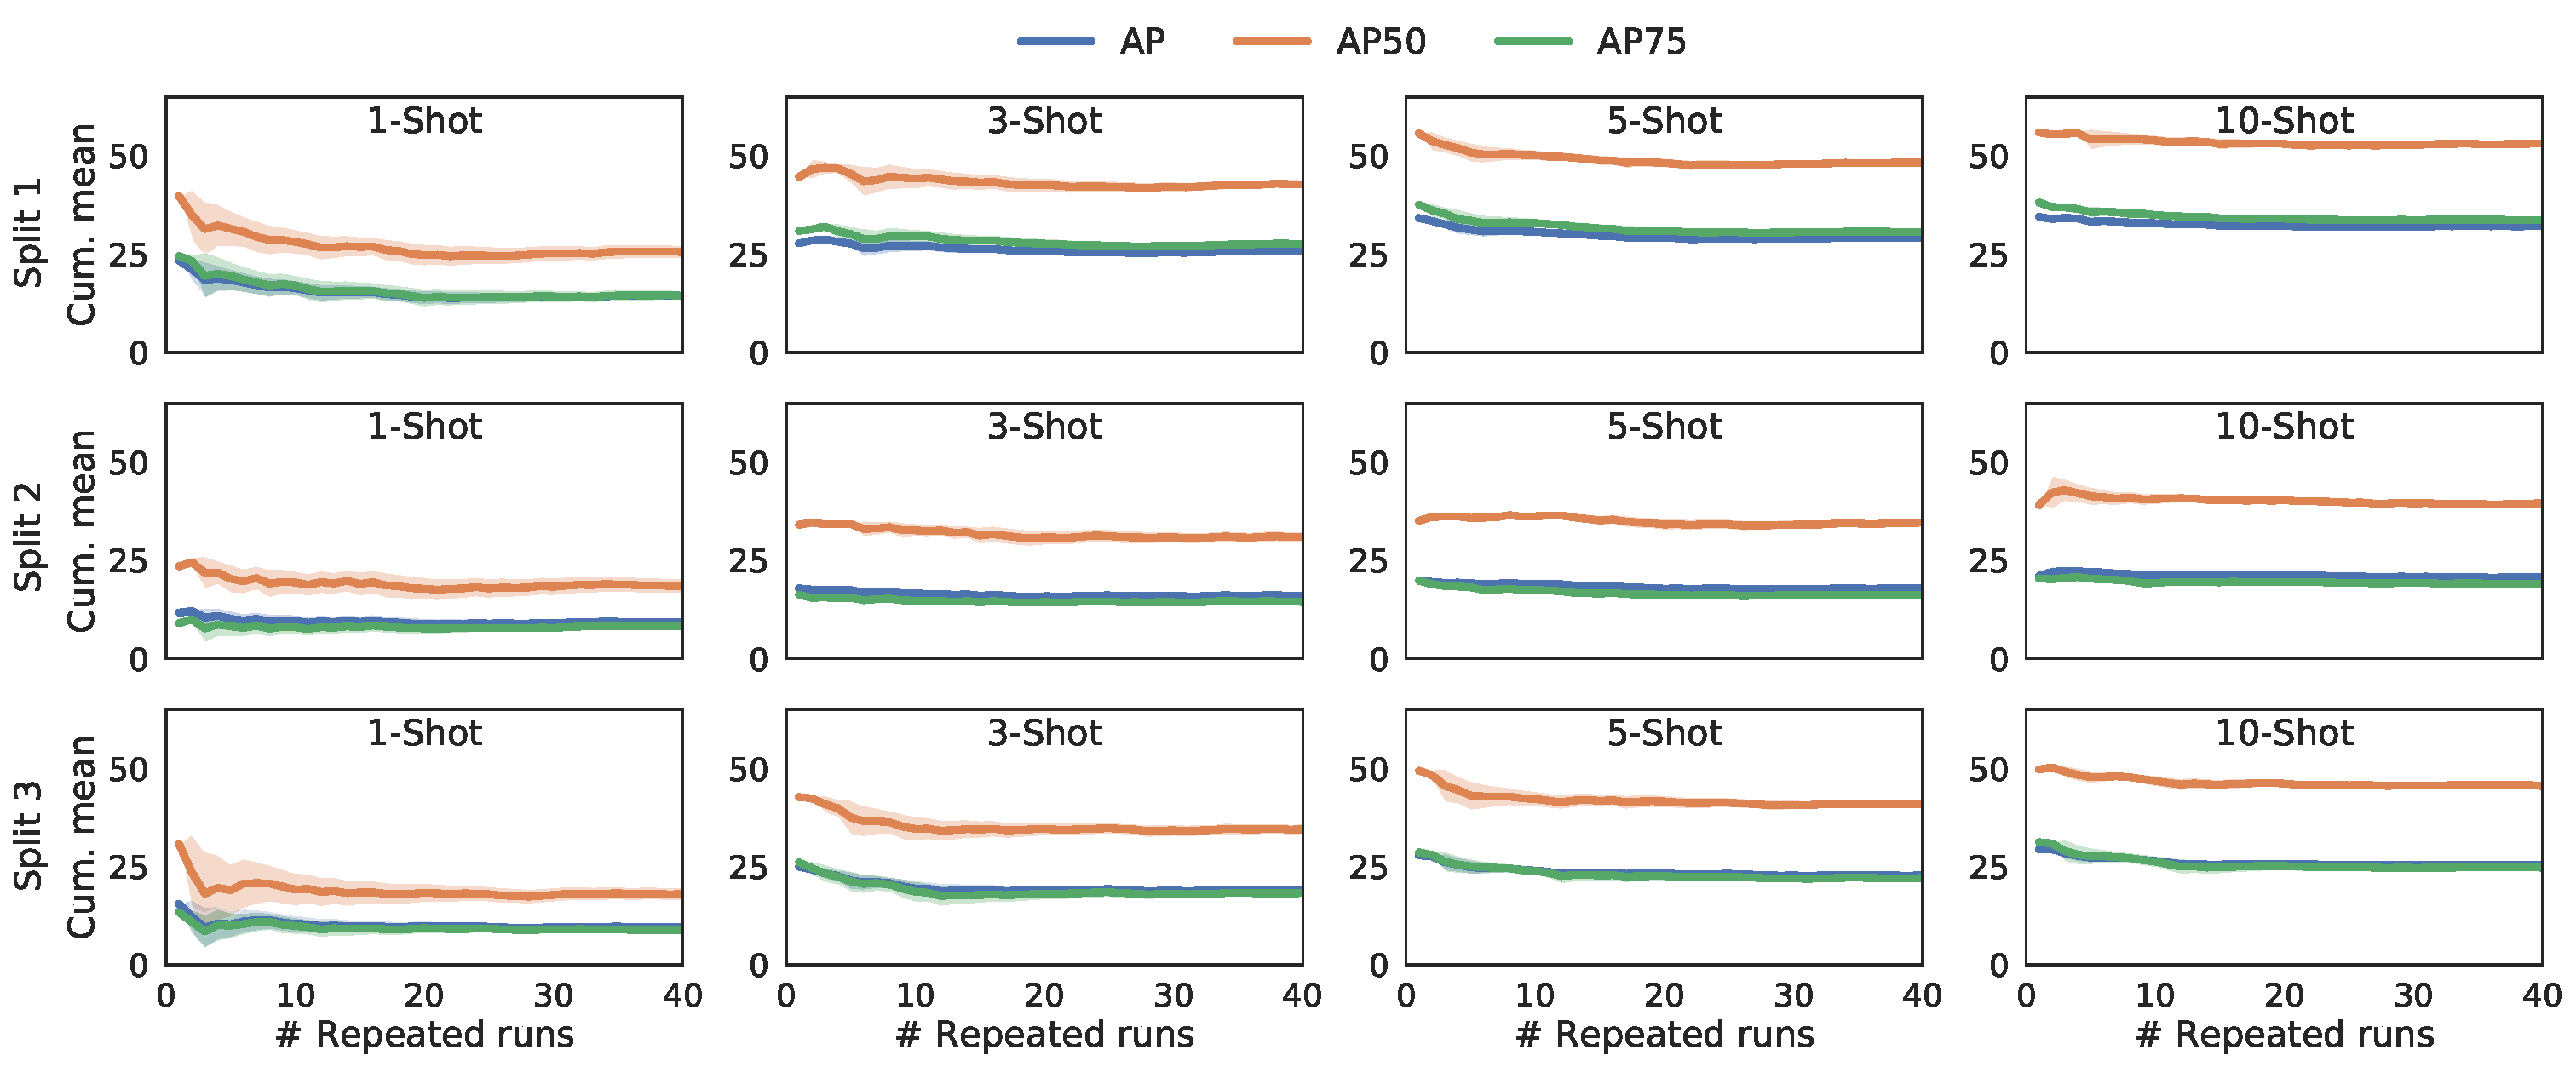
\includegraphics[width=\columnwidth*2]{figs/all_avgap_std.pdf}}
		\vspace{-5mm}
		\caption{Cumulative means with 95\% confidence intervals across 40 repeated runs, computed on the novel classes of all three splits of PASCAL VOC. The means and variances become stable after around 30 runs.}
		\label{fig:avg-ap-sup}
	\end{center}
	\vspace{-10mm}
\end{figure*}

\begin{figure*}[ht]
	\begin{center}
		\centerline{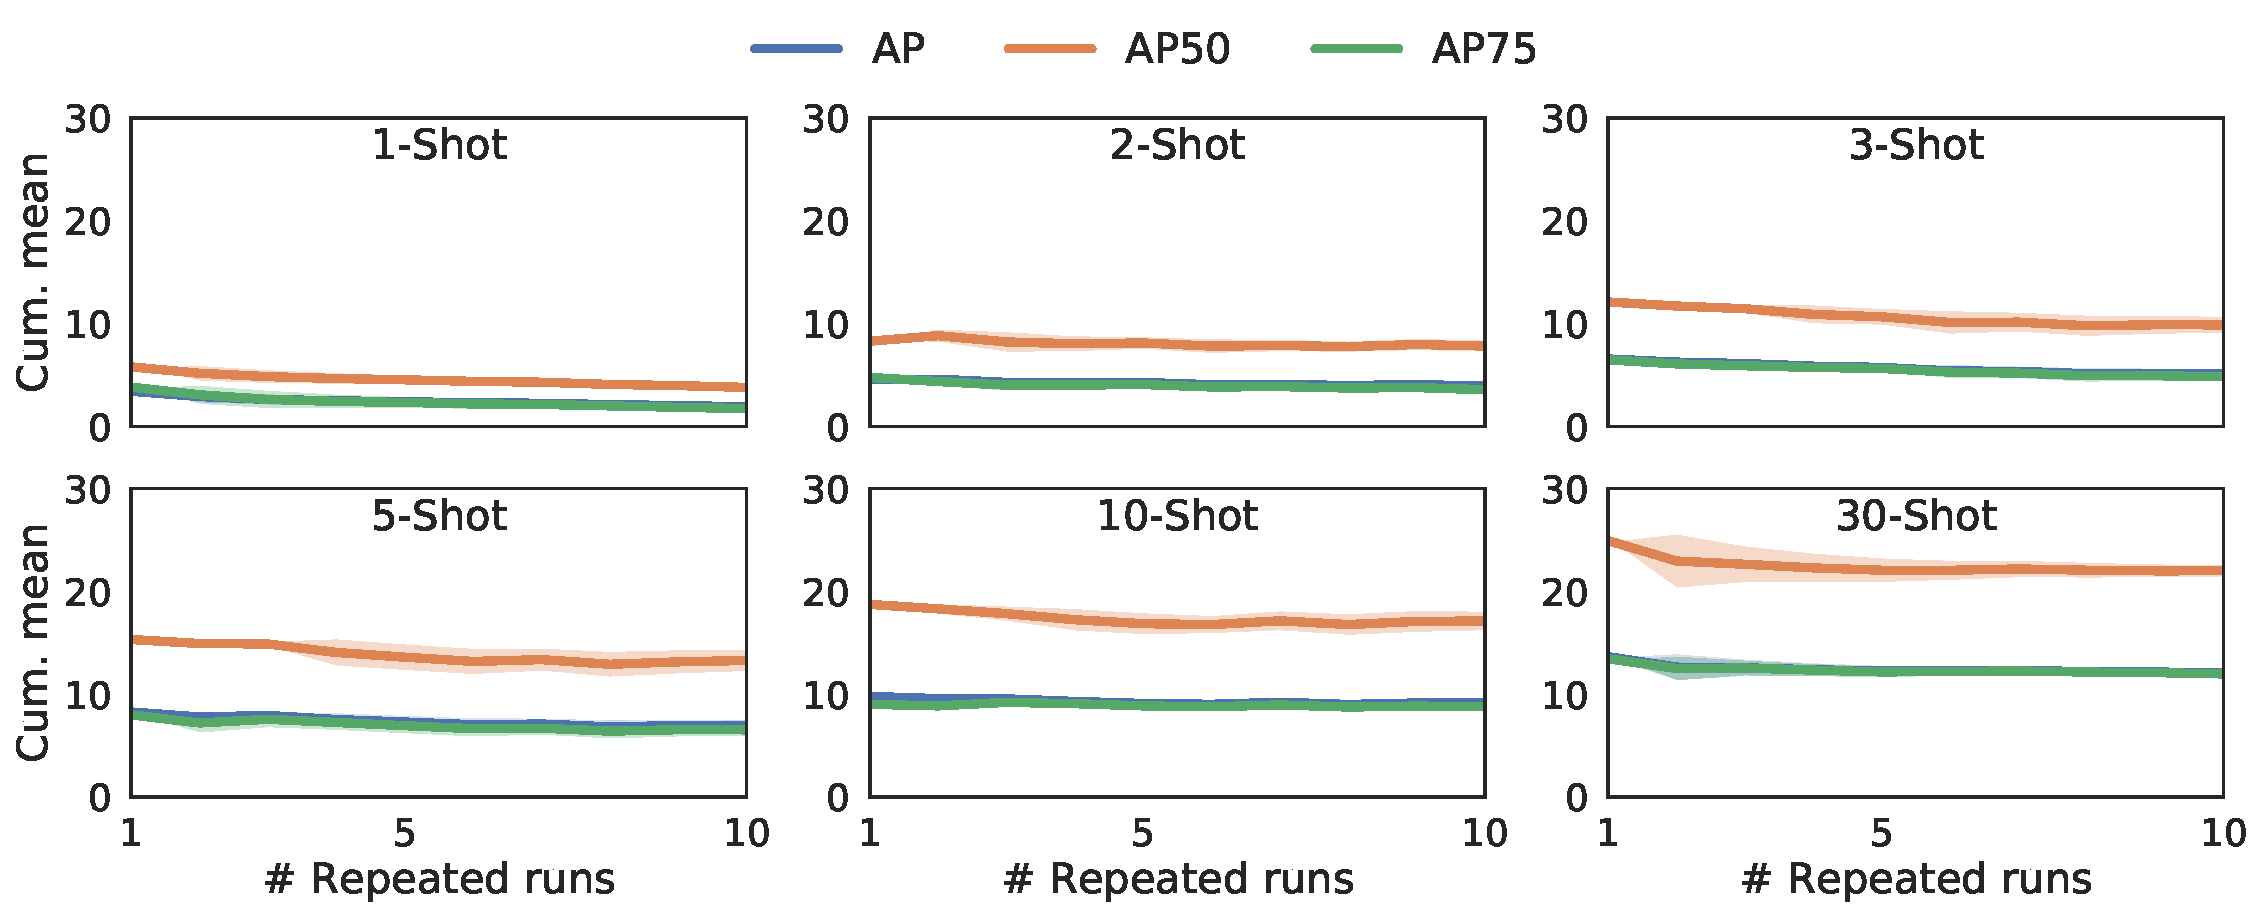
\includegraphics[width=.8\linewidth]{figs/coco_avgap_std.pdf}}
		\vspace{-5mm}
		\caption{Cumulative means with 95\% confidence intervals across 10 repeated runs, computed on the novel classes of COCO.}
		\label{fig:coco-avg-ap-sup}
	\end{center}
	\vspace{-10mm}
\end{figure*}

